\documentclass[a4paper,12pt]{article}
\usepackage[english,russian]{babel}
\usepackage[utf8x]{inputenc}
\usepackage{latexsym,mathrsfs}
\usepackage{stmaryrd, enumitem}
\usepackage{amsthm,amsfonts,amssymb,amsmath}
\usepackage{geometry}
\usepackage{tempora}
\usepackage[pdftex]{graphicx}

\geometry{top=17mm}  \geometry{bottom=20mm}
\geometry{left=17mm} \geometry{right=17mm}
\linespread{1.1}
\parindent=5mm


\def\titleK#1{\begin{center}{\textbf {#1}}\end{center}}
\def\authorK#1{\begin{center}{#1}\end{center}}



\newenvironment{abstractK}{}



\newtheorem{lemma}{Лемма}
\newtheorem{theorem}{Теорема}
\newtheorem{corollary}{Следствие}
\newtheorem{proposition}{Предложение}
\theoremstyle{definition}
\newtheorem{definition}{Определение}
\theoremstyle{definition}
\newtheorem{question}{Вопрос}
\theoremstyle{definition}
\newtheorem{conjecture}{Гипотеза}

%ВАЖНО: Не менять и не добавлять ничего выше этой строки.
%Изменения вносить только внутри окружения \begin{document}\end{document}

\begin{document}

%Название доклада
\titleK{Анализ сдвиговых преобразований в квазигруппах}
%Информация об авторах
\authorK{И. О. Фамилия1$^{1}$, И. О. Фамилия2$^{1}$, И. О. Фамилия3$^{2}$\\
$^{1}$Организация Автора1 и Автора2 \\ $^{2}$Организация Автора3 \\ {\bf E-mail:} email1@g.nsu.ru, email2@g.nsu.ru, email3@gmail.com}
%Текст тезисов доклада 
%Внутри текста можно использовать стандартные команды TeX а также следующие определенные окружения
%Теорема - \begin{theorem}\end{theorem}
%Лемма - \begin{lemma}\end{lemma}
%Следствие - \begin{corollary}\end{corollary}
%Предложение - \begin{proposition}\end{proposition}
%Определение - \begin{definition}\end{definition}
%Вопрос - \begin{question}\end{question}
%Гипотеза - \begin{conjecture}\end{conjecture}
\begin{abstract}
      Аннотация. Краткое описание содержания работы. \\
\\{\bf Ключевые слова:} \textit{ квазигруппа, статистистический тест.} 
 \end{abstract}


\begin{abstractK}

\section{Введение и постановка задачи}

    Тут напишем про то, почему вообще стали такую задачу рассматривать. 
    Можно что-то добавить про шифрование, сохраняющее формат.

\section{Статистистические тесты для подстановок на малых множествах}

\subsection{Используемые статистики и их распределения}

    Тут написать про то, какие статистики для вычислений использовали и какие для них обычные (либо предельные) распределения.

\subsection{Статистическое тестирование гипотез}

   Тут написать про тест хи-квадрат + что делать, когда знаем только среднее.

\subsection{Исследование избыточности тестов}

    Написать про то, как исследовали корреляцию и какие в итоге тесты выбрали.


\section{Квазигруппы}

\subsection{Общие определения}
    Написать про квазигруппы, изотопы, сдвиги и как с их помощью можно генерировать подстановки на маленьких множествах.

\subsection{Способы генерации квазигрупп}
    Написать про то, какие способы использовали мы в работе.


\section{Результаты исследования}


\subsection{Описание эксперимента}

    Написать про то, что проверяем гипотезу о равнораспределенности ``структурированных'' подстановок в множестве всех возможных подстановок.    
    Написать про то, как 
    \begin{itemize}
        \item генерируем квазигруппы, какого размера?
        \item какие сдвиги используем, на какое число элементов сдвигаем?
        \item как порождаем случайные элементы квазигруппы, на которые будем сдвигать?
    \end{itemize}

\subsection{Результаты экспериментов}

    Тут привести таблицы с разбиением на случаи.
    Например, по одной таблице на каждый способ генерации, по столбцам типы сдвигов + число элементов, по строкам~--- номер/название статистического теста.

\section{Выводы и направления дальнейших исследований}

    Написать, что в итоге получилось.
    Почему какие-то тесты завалили?
    Что можно использовать, что нельзя?

    В направление дальнейших исследований:
    \begin{itemize}
        \item попробовать другие, более сложные методы генерации квазигрупп;
        \item попробовать поискать/построить какие-то другие тесты;
        \item подумать о том, как можно обобщать на бОльшие множества, где выписывать подстановку в явном виде замучаешься.
    \end{itemize}

    NB: не забыть оформить список литературы!


{\it Пример курсива.} Можно использовать стандартные команды TeX для форматирования текста.

Формулы в тексте следует окружать знаками: \$\$. 

Пример: $\mathbb{Z}^{n}_{2}$ --- пространство  двоичных векторов длины $n$.

Многострочная формула: {\it алгебраическая нормальная форма (АНФ, полином Жегалкина)} :
$$f(x_1,\ldots,x_n) = \left( \bigoplus_{k=1}^{n} \bigoplus_{i_1,\ldots,i_k}
a_{i_1,\ldots,i_k} \; x_{i_1}\cdot \ldots \cdot x_{i_k} \right)
\oplus a_0,$$
где при каждом $k$ все индексы $i_1,\ldots,i_k$ различны и параметры $a_0, a_{i_1},\ldots,a_{i_k}$ принимают значения 0 или 1. 

Пример теоремы:

\begin{theorem}
Текст теоремы 1.
\end{theorem}   

Ссылка на литературу \cite{bib1}.

Ссылка на рисунок (рис.\ref{fig:image2}).

%Пример вставки картинок
\begin{figure}[h]
\begin{minipage}[h]{0.49\linewidth}
\center{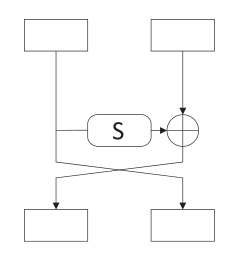
\includegraphics[width=1\linewidth]{feistel.png} }
\caption{Сеть Фейстеля}
\label{fig:image1}
\end{minipage}
\hfill
\begin{minipage}[h]{0.49\linewidth}
\center{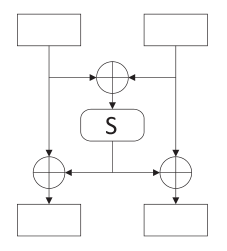
\includegraphics[width=1\linewidth]{laimassey.png} }
\caption{Схема Лая--Месси}
\label{fig:image2}
\end{minipage}
\end{figure}

\newpage
Вставка одиночного рисунка в центре: 

\begin{figure}[h]
\center{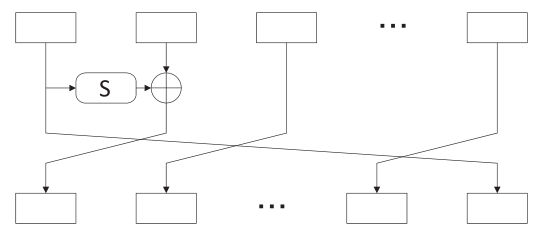
\includegraphics{gfn1.png}}
\caption{Еще схема}
\label{fig:pic3}
\end{figure}

\end{abstractK}
\renewcommand\refname{\center \textnormal{\normalsize{ЛИТЕРАТУРА}}}
%Список литературы
\begin{thebibliography}{}
    \bibitem{bib1} Литература 1.
    \bibitem{bib2} Литература 2.
    \bibitem{bib3} Литература 3.
\end{thebibliography}
\bf{Кураторы исследования
 }-- \rm{\\старший специалист-исследователь Лаборатории Криптографии АО <<НПК <<Криптонит>>, Царегородцев Кирилл Денисович.}
 
\end{document}